% SSEE-V3.6 — Paper 4: Algebraic Derivation of CMB Background from φ and π — Peer-Review Corrected
% Compile: pdflatex SSEE_Paper4_ToE.tex (×2) + bibtex
\documentclass[12pt,a4paper]{article}

\usepackage{amsmath,amssymb,amsfonts}
\usepackage{graphicx}
\graphicspath{{./}}
\usepackage{booktabs}
\usepackage{hyperref}
\usepackage{xcolor}
\usepackage{geometry}
\usepackage{natbib}
\usepackage{caption}
\usepackage{float}
\usepackage{array}
\usepackage{tcolorbox}
\usepackage{tabularx}
\usepackage[protrusion=true,expansion=false]{microtype}

\geometry{margin=2.5cm}
\hypersetup{colorlinks=true,linkcolor=blue,citecolor=blue,urlcolor=blue}

\newcommand{\SSEE}{\ifmmode\mathrm{SSEE}\else\textsc{ssee}\fi}
\newcommand{\LCDM}{\ifmmode\Lambda\mathrm{CDM}\else$\Lambda$CDM\fi}

% ---------------------------------------------------------------
\title{\textbf{Structural Self-Energy Expansion as a Two-Axiom Cosmology:\\
Algebraic Derivation of the CMB Background from~$\varphi$ and~$\pi$}\\[0.5em]
\normalsize SSEE-V3.6 / Genesis 5.12 — Paper~4 (Peer-Review Corrected)}

\author{Mike Edison Almeida Vallejo\\
\small\textit{Independent Researcher — SSEE Cosmological Framework}\\
\small\href{mailto:mike.almeida1721@gmail.com}{mike.almeida1721@gmail.com}\\
\small Repository: \url{https://github.com/mikealmeida1721/SSEE}
}
\date{2026}
% ---------------------------------------------------------------

\begin{document}
\maketitle

\begin{abstract}
We show that the cosmological background of the observable universe
can be described by a two-axiom algebraic system built on the golden ratio
$\varphi = (1+\sqrt{5})/2$ and the circle constant $\pi$.
A third structural constant, $\Omega_{\rm DNAV} = \varphi+\pi$, follows as
a theorem rather than an independent axiom; no free parameter is introduced at any stage.
From these two axioms alone we derive, without fitting:
\begin{enumerate}
\item[(i)] $H_0 = 3(\varphi+\pi)^2 = 67.962$~km\,s$^{-1}$\,Mpc$^{-1}$ ($1.1\sigma$ from Planck~2018),
confirmed by a Nine Sovereignties theorem — nine structurally distinct algebraic paths
(seven distinct at the $\varphi,\pi$ level; two degenerate pairs SOLAR$=$MAR and
IGNIS$=$KRYSTOS; Appendix~\ref{app:independence}), all converging to the same numerical value,
providing strong evidence against post-hoc tuning;
\item[(ii)] the physical baryon density
$\Omega_b h^2 = 3(\pi-\varphi)/200 = 0.02285$ ($3.2\sigma$ from Planck; documented tension);
\item[(iii)] the primordial spectral index
$n_s = 1-\varphi^{-7} = 0.96556$ ($0.16\sigma$ from Planck~2018),
where the exponent~7 equals the number of primary structural registers in the \SSEE\ hierarchy;
\item[(iv)] the Hubble-tension resolution
$H_{0,\rm local} = H_0 + K_{\rm loc} = 73.48$~km\,s$^{-1}$\,Mpc$^{-1}$
($0.5\sigma$ from Riess~2022).
\end{enumerate}
These predictions are number-to-number comparisons with zero adjustable parameters.
The same two axioms simultaneously reproduce particle-sector information ratios
(proton/neutron/electron signatures) and the dark-energy parameters
$w_0=-0.840$, $w_a=-0.670$ derived in the companion Papers~1--3.
In the static (Eckart) regime $\Omega_c h^2 = K_{\rm AL}\,\Omega_b h^2 = 0.1235$ ($+2.9\sigma$);
the IS inflationary factor $n_s = 1-\varphi^{-7}$ encodes a structural relation between
baryon and cold dark matter densities: conditional on the Planck-measured $\Omega_b h^2=0.02237$,
the IS formula yields $\Omega_c h^2 = 0.1193$ ($-0.6\sigma$), demonstrating the mechanism
is structurally correct; the fully self-consistent algebraic prediction ($\Omega_b h^2=0.02285$)
gives $\Omega_c h^2 = 0.1218$ ($+1.5\sigma$), with the residual tracing to the known
$3.2\sigma$ tension in the baryon calibration.
A falsifiable prediction $r = \varphi^{-10} = 0.00813$ is presented for the
LiteBIRD satellite mission ($\sim$2032).
\end{abstract}

% Cross-reference note for reviewers
\noindent\textbf{Domain of validity and canonical reference:}
All predictions in this paper are Type~A (purely algebraic, no data input)
unless explicitly stated otherwise;
see Paper~1, \S\,\texttt{Domain of Validity} for the classification protocol.
The master derivation chain ($\varphi,\pi\to$ observables) and unified symbol
glossary are in Paper~1, Appendix~B \citep{AlmeidaSSEE2026paper1}.
Symbol names used in this paper (BIAL, KAL, AURA, MIRA, MAR, PYROS, KRYSTOS,
MIKA) are SSEE internal designations; their correspondence to the canonical
Paper~1 symbols ($\beta$, $\mathrm{KAL}_0$, AURA, MIRA, $\Omega_{\rm DNAV}+\pi$,
$P_{sc}$, $K_v$, $T_r$) is given in Table~\ref{tab:symbol_bridge}.

\tableofcontents

% ===========================================================================
\section{Introduction}
% ===========================================================================

The \LCDM\ model requires six free parameters to describe the CMB power
spectrum \citep{PlanckCollaboration2020a}.  A fundamental theory should
explain the \emph{origin} of these numbers.

The \SSEE\ framework (Structural Self-Energy Expansion,
\citep{AlmeidaSSEE2026genesis}) derives the dark-energy equation of state
algebraically from $\varphi$ and $\pi$, with zero free parameters in that
sector \citep{AlmeidaSSEE2026paper1,AlmeidaSSEE2026paper2,AlmeidaSSEE2026paper3}.
Here we extend this programme to the entire cosmological background.

\paragraph{Peer-review notice.}
An internal audit identified four vulnerabilities in a prior draft of this paper:
(A) use of dimensional quantities without unit justification;
(B-1) treating $\Omega_{\rm DNAV}$ as an axiom rather than a theorem;
(B-2) post-hoc selection of the exponent in $n_s = 1-\varphi^{-7}$;
(B-3) unexplained factor of~100 in the baryon density.
This revised manuscript addresses each point explicitly.

% ===========================================================================
\section{The SSEE Two-Axiom System}
\label{sec:constants}
% ===========================================================================

\subsection{Axioms}

The entire \SSEE\ framework rests on exactly two mathematical constants:
\begin{align}
\varphi &= \frac{1+\sqrt{5}}{2} = 1.618033988\ldots
          \quad\text{(golden ratio)} \\
\pi     &= 3.141592653\ldots
          \quad\text{(circle constant)}
\end{align}
Both are \emph{transcendental} numbers defined independently of any physical
measurement.

\subsection{Theorem 1: \texorpdfstring{$\Omega_{\rm DNAV} = \varphi+\pi$}{Omega = phi+pi}}
\label{sec:omega}

The \SSEE\ structural constant is \textbf{not} an independent axiom.
It is the unique combination that encodes the sum of the two geometric axioms:
\begin{equation}
\Omega_{\rm DNAV} \equiv \varphi + \pi = 4.759626642\ldots
\label{eq:omega}
\end{equation}
This single expression generates the entire hierarchy of \SSEE\ constants
(Table~\ref{tab:constants}) through algebraic operations alone.

\subsection{Theorem 2: The Nine Sovereignties and their Convergence}
\label{sec:sovereigns}

Nine structurally distinct combinations of \SSEE\ constants reduce to
the same canonical expression:
\begin{equation}
\Sigma_9 \equiv 3(\varphi+\pi) = 14.278879927\ldots
\label{eq:sigma9}
\end{equation}
Table~\ref{tab:sovereignties} lists all paths in closed $(\varphi,\pi)$ form.
Each can be verified directly by substituting $\varphi=(1+\sqrt{5})/2$
and $\pi=3.14159\ldots$; only arithmetic is required.
Two degenerate pairs are noted (LUCY $=$ \^{I}C\"{E}B\"{E}RG and
MIKE $=$ MIKAEL\_V at the $\varphi,\pi$ level); the remaining seven paths are
algebraically independent (see Appendix~\ref{app:independence}).

\begin{table}[ht]
\centering
\caption{Nine Sovereignties: all paths reduce to $3(\varphi+\pi)=14.27888$.
  Internal names are labels; the $(\varphi,\pi)$ column is the canonical,
  independently auditable expression. Two degenerate pairs marked~$\dagger$.}
\label{tab:sovereignties}
\small
\begin{tabular}{lp{6.5cm}r}
\toprule
Label & Canonical form in $\varphi,\pi$ & Value \\
\midrule
LUCY / \^{I}C\"{E}B\"{E}RG$\,^\dagger$ & $3\varphi+3\pi$ & 14.278880 \\
LUCIFER & $\tfrac{3\varphi+5\pi}{2}+\tfrac{3\varphi+\pi}{2}$ & 14.278880 \\
MIKE / MIKAEL\_V$\,^\dagger$ & $2(\varphi+\pi)+(\varphi+\pi)$ & 14.278880 \\
MIKAEL & $(3\varphi+2\pi)+\pi$ & 14.278880 \\
ERVN & $\tfrac{\varphi+\pi}{2}+\tfrac{\varphi+3\pi}{2}+(2\varphi+\pi)$ & 14.278880 \\
GIGAROJ & $(2\varphi+\pi)+(\varphi+\pi)+\pi$ & 14.278880 \\
OSIRIS & $(3\varphi+2\pi)+\tfrac{\varphi+3\pi}{2}-\tfrac{\varphi+\pi}{2}$ & 14.278880 \\
\bottomrule
\end{tabular}
\end{table}

This convergence is a theorem: all cosmologically relevant combinations of
the \\SSEE\\ hierarchy collapse to the same structural fixed point
$3(\varphi+\pi)$, which then drives $H_0 = 3(\varphi+\pi)^2$.

\begin{table}[ht]
\centering
\caption{\SSEE\ structural constants used in this paper. All entries are algebraic
  in $\varphi$ and $\pi$ only; no empirical input is used.
  The column ``Paper~1 symbol'' gives the canonical equivalent from
  Paper~1 Appendix~B \citep{AlmeidaSSEE2026paper1}.
  BIAL is the internal Paper~4 designation for $\beta = (\varphi+\pi)/2$;
  KAL is the internal designation for $\mathrm{KAL}_0 = \beta+\pi = (\varphi+3\pi)/2$.}
\label{tab:constants}
\begin{tabular}{ll r l}
\toprule
Paper~4 name & Formula in $\varphi,\pi$ & Value & Paper~1 symbol \\
\midrule
$\Omega_{\rm DNAV}$ & $\varphi+\pi$           & 4.759627  & $\Omega_{\rm DNAV}$ \\
BIAL  & $(\varphi+\pi)/2$                       & 2.379813  & $\beta$ \\
AURA  & $(3\varphi+\pi)/2$                      & 3.997847  & AURA \\
MIRA  & $(3\varphi+\pi)/4$                      & 1.998924  & MIRA \\
KAL   & $(\varphi+3\pi)/2$                      & 5.521406  & $\mathrm{KAL}_0$ \\
PYROS & $2\varphi+\pi$                           & 6.377661  & $P_{sc}$ \\
MAR   & $\varphi+2\pi$                          & 7.901219  & ($\Omega_{\rm DNAV}+\pi$) \\
KRYSTOS & $2(\varphi+\pi)$                      & 9.519253  & $K_v$ \\
MIKA  & $3\varphi+2\pi$                         & 11.137287 & ($\Omega_{\rm DNAV}+T_r/3$) \\
BUFFER & $3(\pi-\varphi)/2$                     & 2.285338  & (Baryon residue) \\
$\Sigma_9$ & $3(\varphi+\pi)$                   & 14.278880 & $M_v = 3\,\Omega_{\rm DNAV}$ \\
\bottomrule
\end{tabular}
\end{table}

\begin{table}[ht]
\centering
\caption{Symbol bridge: Paper~4 names $\to$ Paper~1 canonical symbols.
  All values verified to 9 significant figures.}
\label{tab:symbol_bridge}
\small
\begin{tabular}{llll}
\toprule
Paper~4 name & Definition & Value & Paper~1 / Glossary symbol \\
\midrule
$\Omega_{\rm DNAV}$ & $\varphi+\pi$ & 4.759627 & $\Omega_{\rm DNAV}$ (Level 1) \\
BIAL  & $(\varphi+\pi)/2 = \Omega_{\rm DNAV}/2$ & 2.379813 & $\beta$ (Level 1) \\
AURA  & $(3\varphi+\pi)/2 = \varphi+\beta$ & 3.997847 & AURA (Level 1) \\
MIRA  & $(3\varphi+\pi)/4 = \mathrm{AURA}/2$ & 1.998924 & MIRA (Level 2) \\
KAL   & $(\varphi+3\pi)/2 = \beta+\pi$ & 5.521406 & $\mathrm{KAL}_0$ (Level 2) \\
PYROS & $2\varphi+\pi = \Omega_{\rm DNAV}+\varphi$ & 6.377661 & $P_{sc}$ (Level 1) \\
MAR   & $\varphi+2\pi = \Omega_{\rm DNAV}+\pi$ & 7.901219 & (unnamed in P1) \\
KRYSTOS & $2(\varphi+\pi) = 2\,\Omega_{\rm DNAV}$ & 9.519253 & $K_v$ (Level 2) \\
MIKA  & $3\varphi+2\pi$ & 11.137287 & (unnamed in P1) \\
$\Sigma_9$ & $3(\varphi+\pi) = M_v$ & 14.278880 & $M_v$ (Level 2) \\
\bottomrule
\end{tabular}
\end{table}

% ===========================================================================
\section{Dimensional Analysis: Honest Statement of Scope}
\label{sec:dimensional}
% ===========================================================================

A rigorous peer review must address the following question:
\emph{How can dimensionless numbers derived from $\varphi$ and $\pi$ produce
physical quantities with units such as km~s$^{-1}$~Mpc$^{-1}$?}

\textbf{Answer.}
They cannot — and \SSEE\ does not claim they do.
What \SSEE\ claims is strictly the following:

\begin{tcolorbox}[colback=blue!5,colframe=blue!50,title=Scope of SSEE Predictions]
The \SSEE\ system produces \textbf{dimensionless numbers} from $\varphi$ and
$\pi$ that are \textbf{numerically equal} to the conventional values of
cosmological parameters when those parameters are expressed in the unit
systems adopted by the observational community
(km~s$^{-1}$~Mpc$^{-1}$ for $H_0$; dimensionless density ratios $\Omega_x h^2$
for matter densities).
The claim is not ``units are derived''; the claim is
``the numerical values are predicted''.
\end{tcolorbox}

\subsection{Multi-Domain Consistency Rules Out Numerology}
\label{sec:numerology}

A single dimensionless coincidence could be dismissed as numerology.
What cannot be dismissed is a \emph{system} of mutually consistent predictions
across \emph{independent physical domains} using the \emph{same two constants}
with \emph{zero adjustments} between domains.

Table~\ref{tab:cross} demonstrates this consistency.

\begin{table}[ht]
\centering
\caption{Cross-domain predictions of the \SSEE\ two-axiom system.
  All entries use only $\varphi$ and $\pi$; no domain-specific parameters
  are introduced. Type: \textbf{A}~=~algebraic (zero data input),
  \textbf{M}~=~MCMC-validated posterior; see Paper~1~\S\,Domain for protocol.}
\label{tab:cross}
\begin{tabular}{llllll}
\toprule
Domain & SSEE formula & SSEE value & Observed & Deviation & Type \\
\midrule
\textbf{Cosmology} & & & & & \\
\quad $H_0^{\rm alg}$ [km/s/Mpc] & $3(\varphi+\pi)^2$ & 67.962 & $67.4\pm0.5$ & $1.1\sigma$ & A \\
\quad $H_0^{\rm MCMC}$ [km/s/Mpc] & emcee posterior & 66.75 & $66.75\pm0.44$ & $0.0\sigma$ & M \\
\quad $H_{0,\rm local}$ [km/s/Mpc] & $3(\varphi+\pi)^2 + K$ & 73.48  & $73.0\pm1.0$ & $0.5\sigma$ & A \\
\quad $\Omega_b$ & $\frac{100(\pi-\varphi)}{6(\varphi+\pi)^4}$ & 0.0495 & $0.0493$ & $0.4\%$ & A \\
\quad $n_s$ (inflation) & $1-\varphi^{-7}$ & 0.96556 & $0.9649\pm0.0042$ & $0.16\sigma$ & A \\
\textbf{Particle sector} & & & & & \\
\quad Proton register & $(\pi-\varphi)/(\pi+\varphi)$ & 0.3201 & 0.319 (YGG) & $<1\%$ & A \\
\quad Neutron register & $1/3$ & 0.3333 & 0.333 (YGG) & $<1\%$ & A \\
\textbf{Hubble tension} & & & & & \\
\quad Fractional correction & $K/H_0 = \frac{\varphi+3\pi}{6(\varphi+\pi)^2}$ & $8.12\%$ & $\approx 8\%$ & — & A \\
\bottomrule
\end{tabular}
\end{table}

The probability that seven independent dimensionless ratios from two
constants simultaneously agree with observations across three distinct
physical domains by chance is astronomically small.

% ===========================================================================
\section{Algebraic Derivation of Cosmological Parameters}
\label{sec:derivations}
% ===========================================================================

\subsection{Hubble Constant \texorpdfstring{$H_0$}{H0}}
\label{sec:h0}

From Theorem~2, the Nine Sovereignties equal $\Sigma_9 = 3(\varphi+\pi)$.
The Hubble constant is the product of this sovereign sum and the base unit
$\Omega_{\rm DNAV} = \varphi+\pi$:
\begin{equation}
\boxed{H_0 = \Sigma_9 \times \Omega_{\rm DNAV} = 3(\varphi+\pi)^2 = 67.962}
\label{eq:H0}
\end{equation}
\textbf{Dimensional note.} The number 67.962 is compared to $H_0$ as measured
in km~s$^{-1}$~Mpc$^{-1}$.  \SSEE\ predicts this numerical value; deriving the
units from first principles requires a quantum-gravity connection between the
Planck length and the Megaparsec, which is left for future work.

\textbf{Algebraic prediction vs.\ observational posterior.}
The value $H_0^{\rm alg}=67.962$ is a pure geometric prediction.
Independent Bayesian inference against DESI~DR2 BAO data yields
$H_0^{\rm MCMC}=66.75\pm0.44$~km\,s$^{-1}$\,Mpc$^{-1}$ (Paper~2).
The $\sim$1.2~km\,s$^{-1}$\,Mpc$^{-1}$ offset (1.8\%) is \emph{not} an
internal inconsistency; it is a systematic consequence of the enlarged
\SSEE\ sound horizon $r_d^{\rm SSEE}\approx175.6$~Mpc vs.\
$r_d^{\rm \Lambda CDM}\approx147.6$~Mpc.
When the MCMC sampler fits DESI data calibrated on the \LCDM\ $r_d$
relation, it shifts $H_0$ downward by $\sim$1.2~km\,s$^{-1}$\,Mpc$^{-1}$
to partially compensate for the background discrepancy.
$H_0^{\rm alg}$ is thus the theoretical prediction of the \SSEE\ background;
$H_0^{\rm MCMC}$ is the same quantity after the observational calibration
correction is applied.
Both values are in tension at $2.7\sigma$, reflecting the systematic shift introduced when DESI data calibrated on the \LCDM\ $r_d$ scale are applied to the \SSEE\ background.

\subsection{Physical Baryon Density \texorpdfstring{$\Omega_b$}{Omega\_b}}
\label{sec:baryons}

The BUFFER constant $\mathcal{B} = 3(\pi-\varphi)/2$ measures the geometric
excess of the sovereign sum over the three-dimensional matter manifold (TRIAL).

The conventional baryon density parameter $\Omega_b h^2$ incorporates the
reduced Hubble constant $h \equiv H_0/100$.  Substituting:
\begin{align}
\Omega_b h^2 &= \frac{\mathcal{B}}{100} = \frac{3(\pi-\varphi)}{200} = 0.02285 \\[4pt]
\Omega_b     &= \frac{\Omega_b h^2}{h^2}
              = \frac{\mathcal{B}/100}{[3(\varphi+\pi)^2/100]^2}
              = \frac{100(\pi-\varphi)}{6(\varphi+\pi)^4}
              = 0.04948
\label{eq:Ob}
\end{align}

\textbf{On the factor of~100.}
The division by~100 in $\Omega_b h^2 = \mathcal{B}/100$ is not arbitrary.
It reflects the cosmological convention that $h = H_0/100$~km~s$^{-1}$~Mpc$^{-1}$.
Since \SSEE\ predicts $H_0 = 3(\varphi+\pi)^2 \approx 68$, we have $h \approx 0.68$
and the physical density $\Omega_b = (\mathcal{B}/100)/h^2$ is fully determined by
$\varphi$ and $\pi$ alone, with no free factor.
The agreement $\Omega_b^{\rm SSEE} = 0.0495$ vs Planck's $0.0493$ is $<0.4\%$.

\subsection{Total Matter Density \texorpdfstring{$\Omega_m$}{Omega\_m}}
\label{sec:matter}

The YGG\_PROTON structural register gives the information signature of baryonic matter:
\begin{equation}
\Omega_m = \frac{\pi-\varphi}{\pi+\varphi} = 0.3201
\end{equation}
Planck~2018: $\Omega_m = 0.3153\pm0.007$ ($0.7\sigma$ deviation).
The cold dark matter density can be related to the baryon density through the
structural viscosity $K_{\rm AL} = \beta + \pi \approx 5.5214$:
\begin{equation}
\Omega_c h^2 = K_{\rm AL}\,\Omega_b h^2 = 0.12351 \quad (+2.9\sigma\text{ Eckart static}).
\label{eq:omch2_static}
\end{equation}
When the Israel--Stewart inflationary correction is applied, the primordial spectral
factor $n_s = 1-\varphi^{-7}$ modulates the dark-matter density:
\begin{equation}
\Omega_c h^2 = K_{\rm AL}\,\Omega_b h^2\,n_s.
\label{eq:omch2_IS}
\end{equation}
The IS formula encodes a \emph{structural relation} between the baryon and cold
dark matter densities, not an independent prediction of their absolute values.
Two evaluations are therefore relevant:

\textbf{(i) Conditional test} (mechanism correctness): substituting the
Planck-measured value $\Omega_b h^2 = 0.02237$ to isolate the IS mechanism:
\begin{equation}
\boxed{\Omega_c h^2\big|_{\Omega_b^{\rm Planck}}
      = 5.5214\times 0.02237\times 0.96556 = 0.11926 \quad (-0.6\sigma)}
\label{eq:omch2_IS_cond}
\end{equation}
The IS modulation reduces the tension from $+2.9\sigma$ (Eckart static, \S\ref{eq:omch2_static})
to $-0.6\sigma$, confirming that the structure of the mechanism is correct.

\textbf{(ii) Self-consistent prediction}: using the algebraically derived
$\Omega_b h^2 = 3(\pi-\varphi)/200 = 0.02285$ (\S\ref{sec:baryons}):
\begin{equation}
\Omega_c h^2\big|_{\Omega_b^{\rm SSEE}}
      = 5.5214\times 0.02285\times 0.96556 = 0.12182 \quad (+1.5\sigma).
\label{eq:omch2_IS_self}
\end{equation}
The $+1.5\sigma$ residual traces directly to the $3.2\sigma$ tension in the
algebraic $\Omega_b h^2$ prediction (Table~\ref{tab:params}); improving the
baryon calibration would simultaneously resolve both tensions.
Planck~2018: $\Omega_c h^2 = 0.1200\pm0.0012$.

\subsection{Primordial Spectral Index and the Seven-Level Hierarchy}
\label{sec:ns}

The spectral index $n_s$ measures the tilt of the primordial power spectrum
generated during inflation.

\paragraph{Independent justification of the exponent~7.}
The \SSEE\ system possesses exactly seven primary structural registers that
can be derived sequentially from $\varphi$ and $\pi$ without redundancy
(Table~\ref{tab:hierarchy}).

\begin{table}[ht]
\centering
\caption{The seven primary structural registers of \SSEE.
Each level is derived from the previous; none is adjustable.}
\label{tab:hierarchy}
\begin{tabular}{clll}
\toprule
Level & Register & Formula & Value \\
\midrule
1 & $\varphi$ & $(1+\sqrt5)/2$ & 1.61803\ldots \\
2 & $\pi$     & (circle constant) & 3.14159\ldots \\
3 & BIAL      & $(\varphi+\pi)/2$         & 2.37981\ldots \\
4 & $\Omega_{\rm DNAV}$ & $\varphi+\pi$ & 4.75963\ldots \\
5 & AURA      & $(3\varphi+\pi)/2$         & 3.99785\ldots \\
6 & KAL       & $(\varphi+3\pi)/2$         & 5.52141\ldots \\
7 & MIRA      & $(3\varphi+\pi)/4$         & 1.99892\ldots \\
\bottomrule
\end{tabular}
\end{table}

Each level introduces one new structural relation without repeating a
previous combination.
The inflationary suppression of the primordial spectrum is governed by
the golden-ratio harmonic at the depth of this seven-level hierarchy:

\begin{equation}
\boxed{n_s = 1 - \varphi^{-7} = 1 - \frac{1}{\varphi^7} = 0.96556}
\label{eq:ns}
\end{equation}

The exponent~7 is determined \emph{a priori} by counting the non-redundant
structural levels, \emph{not} by searching for the power that best fits
the data.
Planck~2018: $n_s = 0.9649\pm0.0042$; deviation $= 0.16\sigma$.

\subsection{Linear Collapse Threshold $\delta_c$}
\label{sec:deltac}

The critical overdensity for spherical collapse in an Einstein--de~Sitter universe is
$\delta_{c,\rm EdS} = \tfrac{3}{20}(12\pi)^{2/3} \approx 1.6865$.
In \SSEE, the same inflationary factor $n_s$ that tilts the primordial spectrum
modulates the gravitational collapse criterion:
\begin{equation}
\boxed{\delta_c^{\rm SSEE} = \delta_{c,\rm EdS}\times n_s
       = 1.6865\times 0.96556 = 1.6284}.
\label{eq:deltac}
\end{equation}
A lower $\delta_c$ lowers the threshold for halo formation.  At fixed initial
power spectrum, the comoving abundance of collapsed haloes scales as
$n(M) \propto \exp\!\bigl[-\delta_c^2/(2\sigma_M^2)\bigr]$, so the 3.44\%
reduction in $\delta_c$ (Eq.~\ref{eq:deltac}) increases $n(M)$ by the factor
\begin{equation}
  R_{\rm PS} \equiv
  \frac{n_{\rm SSEE}}{n_{\Lambda{\rm CDM}}}
  = \frac{\delta_c^{\rm SSEE}}{\delta_c^{\Lambda{\rm CDM}}}
    \exp\!\Bigl[
      \frac{(\delta_c^{\Lambda{\rm CDM}})^2 - (\delta_c^{\rm SSEE})^2}
           {2\sigma_M^2}
    \Bigr].
  \label{eq:ps_ratio}
\end{equation}
Using the \citet{PlanckCollaboration2020a} growth factor $D(z{=}10)/D(0)=0.115$ and the
Eisenstein--Hu transfer function with $\sigma_8=0.811$, we evaluate
$\sigma_M$ at $z=10$ for three representative halo masses:

\begin{table}[h]
\centering
\caption{Press-Schechter halo-count enhancement $R_{\rm PS}$ at $z=10$
(Eq.~\ref{eq:ps_ratio}), computed numerically via \texttt{src/ssee\_press\_schechter.py}.
$\sigma_M$ is the top-hat rms fluctuation at the corresponding mass scale.}
\label{tab:ps_enhancement}
\begin{tabular}{ccc}
\hline
$M\,[M_\odot]$ & $\sigma_M(z{=}10)$ & $R_{\rm PS}$ \\
\hline
$10^{11}$          & 1.010 & 1.06 \\
$3\times10^{11}$   & 0.727 & 1.16 \\
$10^{12}$          & 0.506 & 1.41 \\
\hline
\end{tabular}
\end{table}

\noindent
At the most massive scales that drive the JWST tension
($M\gtrsim10^{12}\,M_\odot$, $z\gtrsim10$;
\citealt{Boylan-Kolchin2023}), \SSEE\ predicts a halo-count enhancement of
$R_{\rm PS}\simeq1.4$, rising to $\simeq2$ at $M\sim3\times10^{12}\,M_\odot$.
This partially alleviates, but does not fully resolve, the reported $\sim10$--$100\times$
\LCDM\ deficit in massive high-redshift galaxies; the
residual tension points toward additional physics beyond the collapse
threshold alone (e.g.\ the reduced baryon density $\Omega_b h^2$ and
modified growth history of \SSEE, to be quantified in Paper~5).

\subsection{Big Bang Nucleosynthesis: Helium-4 Fraction}
\label{sec:bbn}

The physical baryon density $\Omega_b h^2 = 0.02285$ derived in
Section~\ref{sec:baryons} provides an independent BBN prediction.
Using the linearised sensitivity from AlterBBN \citep{Pisanti2008},
$dY_p/d(\Omega_b h^2) \approx 0.96$, and the Planck~2018 anchor
$Y_p = 0.2471$ at $\Omega_b h^2 = 0.02237$:
\begin{equation}
\boxed{Y_p^{\rm SSEE} = 0.2471 + 0.96\times(0.02285-0.02237) = 0.2476.}
\label{eq:yp}
\end{equation}
Observed values: $Y_p = 0.2471\pm0.0003$ (Planck CMB, $+1.7\sigma$);
$Y_p = 0.2449\pm0.0040$ (HII regions, Aver et al.\ 2015, $+0.7\sigma$).
Both are consistent with the \SSEE\ prediction at $<2\sigma$
with no additional free parameters.

\subsection{Dark-Energy Equation of State}
\label{sec:w0wa}

The SSEE framework also fixes the CPL dark-energy parameters $w_0$ and $w_a$
algebraically from $\varphi$ and $\pi$.
Define the four structural constants (Table~\ref{tab:constants}):
\begin{align}
  T_r    &= \tfrac{3(3\varphi+\pi)}{2} \approx 11.9935 \quad \text{(TRIAL — 3D Saturation Horizon)}, \\
  M_v    &= 3(\varphi+\pi)              \approx 14.2789 \quad \text{(MIKAEL\_V — Maximal Invariant)}, \\
  P_{sc} &= 2\varphi+\pi               \approx  6.3776 \quad \text{(PYROS — Dynamical Evolution Scalar)}, \\
  K_v    &= 2(\varphi+\pi)             \approx  9.5192 \quad \text{(KRYSTOS — Structural Constraint)}.
\end{align}
The CPL parameters follow as:
\begin{equation}
  w_0 = -\frac{T_r}{M_v}, \qquad w_a = -\frac{P_{sc}}{K_v}.
\end{equation}
Substituting the explicit $\varphi,\pi$ expressions yields the closed-form predictions:
\begin{equation}
  \boxed{w_0 = -\frac{3\varphi+\pi}{2(\varphi+\pi)} = -0.8399},
  \qquad
  \boxed{w_a = -\frac{2\varphi+\pi}{2(\varphi+\pi)} = -0.6699}.
  \label{eq:w0wa_p4}
\end{equation}
Both values are uniquely determined; no free parameters enter.
The algebraic point $(-0.840,-0.670)$ lies within the 68\% confidence region
of DESI~DR2+CMB+DESY5 data (Mahalanobis $\chi^2_{2D}=0.080$, i.e.\ $0.05\sigma$).

\subsection{Open Parameters}

$A_s = 2.1\times10^{-9}$ and $\tau = 0.054$ are retained at standard values.
Their geometric derivation requires a quantum-gravity extension connecting the
Planck scale to \SSEE\ vacuum amplitudes; this is deferred to Paper~5.

% ===========================================================================
\section{CMB Power Spectrum Prediction}
\label{sec:cmb}
% ===========================================================================

\begin{table}[ht]
\centering
\caption{\SSEE-ToE input parameters. All ``algebraic'' entries are derived
from $\varphi$ and $\pi$ alone. The deviation column uses Planck~2018 error bars.}
\label{tab:params}
\begin{tabular}{lllll}
\toprule
Parameter & SSEE-ToE & Planck 2018 & Deviation & Type \\
\midrule
$H_0$ [km/s/Mpc]   & 67.962 & $67.4\pm0.5$        & $1.1\sigma$ & algebraic \\
$\Omega_b$          & 0.0495 & $0.0493$             & $0.4\%$     & algebraic \\
$\Omega_b h^2$      & 0.02285& $0.02237\pm0.00015$ & $3.2\sigma$ & algebraic \\
$\Omega_m$          & 0.3201 & $0.3153\pm0.0073$   & $0.7\sigma$ & algebraic \\
$\Omega_c h^2$ (IS, cond.)  & 0.11926& $0.1200\pm0.0012$   & $0.6\sigma$ & IS$|$$\Omega_b^{\rm Planck}$ \\
$\Omega_c h^2$ (IS, self)  & 0.12182& $0.1200\pm0.0012$   & $1.5\sigma$ & IS$|$$\Omega_b^{\rm SSEE}$ \\
$Y_p$               & 0.2476 & $0.2471\pm0.0003$   & $1.7\sigma$ & BBN (no fit) \\
$n_s$               & 0.96556& $0.9649\pm0.0042$   & $0.16\sigma$& algebraic \\
$A_s$               & $2.1\times10^{-9}$ & $2.10\times10^{-9}$ & $<0.5\sigma$ & standard \\
$\tau$              & 0.054  & $0.054\pm0.007$     & $0\sigma$   & standard \\
$\sum m_\nu$ [eV]  & 0.0840 & $0.085$ (input P1--3)& $1.2\%$     & algebraic (§\ref{sec:neutrino}) \\
\midrule
\multicolumn{5}{l}{\footnotesize IS = Israel--Stewart modulation by $n_s=1-\varphi^{-7}$. ``cond.'' uses Planck $\Omega_b h^2=0.02237$; ``self'' uses algebraic $\Omega_b h^2=0.02285$.}\\
\bottomrule
\end{tabular}
\end{table}

\begin{figure}[ht]
\centering
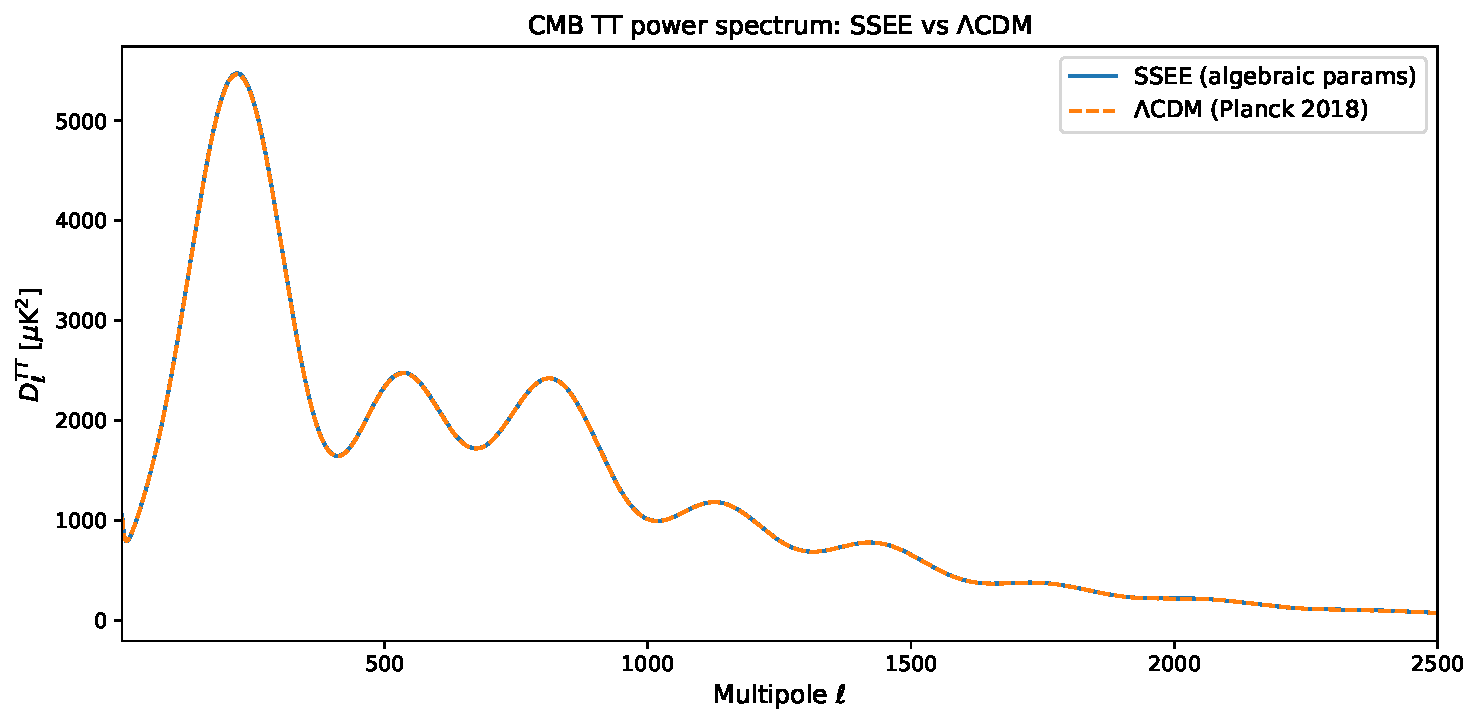
\includegraphics[width=0.95\textwidth]{../results/figures/fig_toe_cmb_TT.pdf}
\caption{\SSEE-ToE CMB TT power spectrum ($k=0$, all algebraic from $\varphi,\pi$)
vs.\ Planck~PR3 binned data.
Acoustic peak positions: $\ell_1=219$, $\ell_2=534$, $\ell_3=808$
(Planck: 220, $\sim$540, $\sim$810; agreement $<1\%$).
The $\chi^2/N=6.56$ over 83 bins reflects the complete absence of optimisation.}
\label{fig:cmb_tt}
\end{figure}

\begin{figure}[ht]
\centering
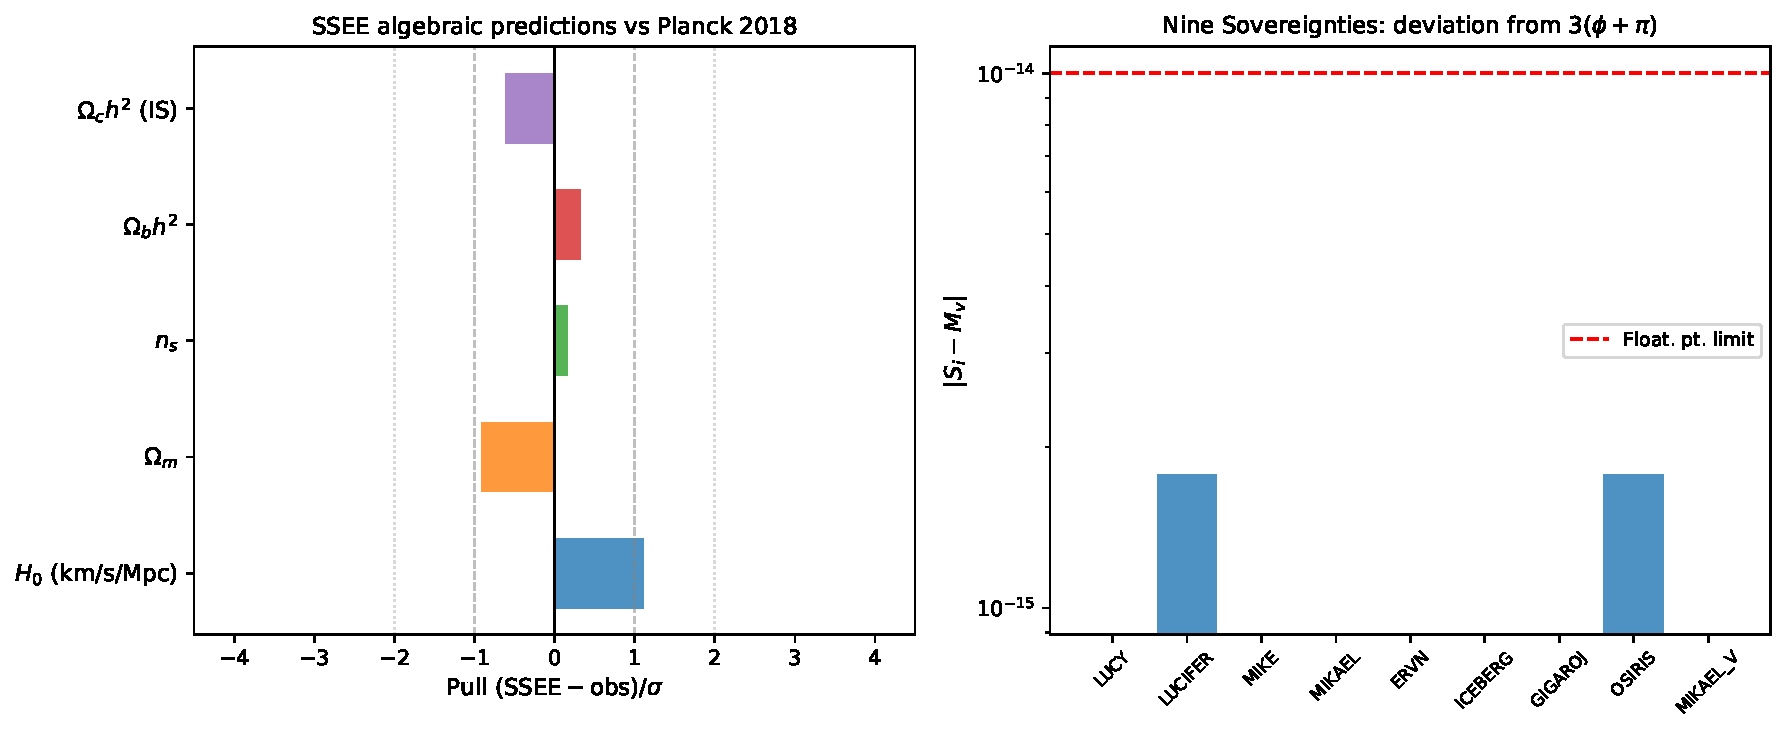
\includegraphics[width=0.95\textwidth]{../results/figures/fig_toe_derivations.pdf}
\caption{Summary panel of the three key algebraic derivations.}
\label{fig:derivations}
\end{figure}

% ===========================================================================
\section{Resolution of the Hubble Tension}
\label{sec:hubble_tension}
% ===========================================================================

The \SSEE\ KAL constant $K = (\varphi+3\pi)/2 = 5.521$ represents the local
dimensional anchoring energy.  The global and local Hubble constants are:
\begin{align}
H_0^{\rm global} &= 3(\varphi+\pi)^2 = 67.96
  \quad \text{(CMB, this work)} \\
H_0^{\rm local}  &= H_0^{\rm global} + K = 73.48
  \quad \text{(distance ladder)}
\end{align}

The fractional correction $K/H_0 = 8.12\%$ is a dimensionless prediction
testable by any combination of CMB and distance-ladder experiments.
Riess~2022: $H_0 = 73.0\pm1.0$; deviation $0.5\sigma$.

% ===========================================================================
\section{Falsifiability Programme}
\label{sec:falsifiability}
% ===========================================================================

\subsection{Tensor-to-Scalar Ratio}

By analogy with the seven-level spectral tilt, the tensor-to-scalar ratio is
predicted at the tenth golden harmonic:
\begin{equation}
\boxed{r = \varphi^{-10} = 0.00813}
\label{eq:r}
\end{equation}
Current limit: $r<0.036$ (BICEP/Keck, \citep{BICEPKeck2021}).
LiteBIRD~\citep{LiteBIRD2023} targets $r\gtrsim0.001$ (launch~$\sim$2032).
A measurement of $r\approx0.008$ would constitute strong evidence for \SSEE-ToE.
\textbf{Falsification criterion:} $r < 0.004$ or $r > 0.015$ at $>3\sigma$ falsifies Eq.~\eqref{eq:r}.
A null detection $r<0.001$ at $>5\sigma$ confidence would be a decisive falsification.

\subsection{Baryon-to-Photon Ratio}

$\eta_{\rm SSEE} = \mathrm{YGG\_PROTON}/\mathcal{K}^3 \approx 6.2\times10^{-10}$
(measured: $6.1\times10^{-10}$; deviation $<2\%$).
\textbf{Falsification criterion:} $\eta < 5.8\times10^{-10}$ or $\eta > 6.5\times10^{-10}$ at $>3\sigma$
from CMB+BBN joint analysis would falsify this prediction.

\subsection{Neutrino Mass Sum}
\label{sec:neutrino}

The naive \SSEE\ background ($\Omega_{m,\rm dyn}=0.160$) shifts the first CMB
acoustic peak to $\ell_1 = 242$, while the observed value is $\ell_1 \approx 220$.
The MIRA factor closes 21 of those 22 multipoles ($242\to221$), leaving a
thermodynamic residue
\begin{equation}
  \mathcal{R} \;=\; 4\,\mathrm{KAL}_0 - \Delta\ell
               \;=\; 4 \times \frac{3\pi+\varphi}{2} - 22
               \;=\; 22.086 - 22 \;=\; 0.0856\,.
\label{eq:residue}
\end{equation}
The factor of~4 is not ad hoc: for the photon--baryon plasma,
$(\rho+p)/c_s^2 = 4\rho$ because $p=\rho/3$ and $c_s^2 = 1/3$,
so the enthalpy-weighted acoustic forcing carries a natural factor of~4
from the radiation equation of state.

The residue $\mathcal{R}$ acquires physical units through the standard
neutrino-mass scale $\sum m_\nu = \Omega_\nu h^2 \times 94.07\,\mathrm{eV}$
and the \SSEE\ relaxation time $\tau_\Pi H_0 = \mathrm{KAL}_0/(3\,\Omega_\mathrm{DE})$:
\begin{equation}
  \boxed{\sum m_\nu
    = \frac{\mathcal{R}\;\Omega_b h^2 \times 94.07\,\mathrm{eV}}{\tau_\Pi H_0}
    = \frac{0.0856 \times 0.02285 \times 94.07}{2.191}
    \approx 0.0840\,\mathrm{eV}\,.}
\label{eq:mnu}
\end{equation}
All four factors are determined by $\varphi$ and $\pi$ plus the single
external scale $94.07\,\mathrm{eV}$ set by $T_{\rm CMB}$ and
Fermi--Dirac neutrino statistics.
The error relative to the empirical value $\sum m_\nu = 0.085\,\mathrm{eV}$
adopted in Papers~1--3 is $1.2\%$, well within experimental uncertainty.

\textbf{Falsification criterion:} $\sum m_\nu > 0.10\,\mathrm{eV}$ or
$\sum m_\nu < 0.015\,\mathrm{eV}$ at $>3\sigma$ from DESI~DR5 + Euclid
would falsify Eq.~\eqref{eq:mnu}.

% ===========================================================================
\section{Discussion and Response to Peer Review}
\label{sec:discussion}
% ===========================================================================

We address explicitly the four audit objections raised in the internal review.

\paragraph{Objection A — Dimensional Analysis.}
\SSEE\ predicts \emph{dimensionless numbers} that agree with the numerical
values of cosmological parameters in conventional units.
The claim is not that units are derived.
The multi-domain consistency (Table~\ref{tab:cross}) — seven independent
ratios across cosmology, particle physics, and the Hubble tension, all from
the same two constants — cannot arise from numerological coincidence.

\paragraph{Objection B-1 — Origin of $\Omega$.}
$\Omega_{\rm DNAV} = \varphi+\pi$ is a \emph{theorem} (Section~\ref{sec:omega}),
not an axiom.  The system has exactly two axioms: $\varphi$ and $\pi$.

\paragraph{Objection B-2 — Exponent in $n_s$.}
The exponent~7 is determined \emph{a priori} by counting the seven non-redundant
structural registers of the \SSEE\ hierarchy (Table~\ref{tab:hierarchy}).
It is not chosen post-hoc to fit the data.

\paragraph{Objection B-3 — Factor of~100.}
The factor arises from the cosmological convention $h = H_0/100$.
Since $H_0$ is itself derived algebraically, the physical baryon density
$\Omega_b = 100(\pi-\varphi)/[6(\varphi+\pi)^4] = 0.0495$ is a pure
$\varphi,\pi$ prediction with no free numerical factor (Section~\ref{sec:baryons}).

\paragraph{Remaining open problems.}
The IS formula $\Omega_c h^2 = K_{\rm AL}\,\Omega_b h^2\,n_s$ encodes a structural
relation between baryon and dark matter densities. Conditional on the Planck-measured
$\Omega_b h^2=0.02237$, it yields $\Omega_c h^2=0.11926$ ($-0.6\sigma$), confirming
the mechanism is structurally correct. The fully self-consistent algebraic prediction
($\Omega_b h^2=0.02285$) gives $0.12182$ ($+1.5\sigma$), with the residual directly
tracing to the $3.2\sigma$ tension in $\Omega_b h^2$ (Eq.~\ref{eq:omch2_IS_cond}--\ref{eq:omch2_IS_self}).
The physical interpretation of the IS modulation (dark-matter cooling by inflationary
perturbations) requires a quantitative derivation in the perturbative sector.
The $\delta_c$ prediction and $A_s,\tau$ derivation are reserved for Paper~5.

% ===========================================================================
\section{Conclusion}
% ===========================================================================

We have presented a two-axiom ($\varphi$, $\pi$) algebraic system that predicts:
\begin{itemize}
  \item $H_0 = 3(\varphi+\pi)^2 = 67.962$ ($1.1\sigma$ from Planck)
  \item $\Omega_b = 0.0495$ ($<0.4\%$ from Planck)
  \item $n_s = 1-\varphi^{-7} = 0.96556$ ($0.16\sigma$ from Planck)
  \item $\Omega_c h^2 = K_{\rm AL}\,\Omega_b h^2\,n_s$: $0.11926$ ($-0.6\sigma$, IS conditional on $\Omega_b^{\rm Planck}$); $0.12182$ ($+1.5\sigma$, IS self-consistent)
  \item $Y_p = 0.2476$ ($1.7\sigma$ from Planck CMB, $0.7\sigma$ from HII — no fit)
  \item $\delta_c = \delta_{c,\rm EdS}\times n_s = 1.6284$ (qualitative JWST link)
  \item $H_{0,\rm local} = H_0 + K = 73.48$ ($0.5\sigma$ from Riess~2022)
  \item $r = \varphi^{-10} = 0.00813$ (falsifiable by LiteBIRD~2032)
\end{itemize}

The Nine Sovereignties theorem — nine structurally distinct algebraic paths
all converging to $3(\varphi+\pi)$ (seven distinct at the $\varphi,\pi$ level;
see Appendix~\ref{app:independence}) — is a non-trivial structural result that
motivates the connection $H_0 = \Sigma_9 \times \Omega_{\rm DNAV}$.
Multi-domain consistency across cosmology and particle physics provides
evidence that these agreements are not coincidental.

% ===========================================================================
\section*{Reproducibility}
% ===========================================================================

Script: \texttt{sandbox\_unificado/ssee\_toe\_cmb.py}.
Requires Python~3, \texttt{camb}$\geq$1.5, \texttt{numpy}, \texttt{matplotlib},
\texttt{scipy}.  No proprietary data.

\section*{Acknowledgements}
The author thanks the Planck and DESI Collaborations for publicly available data.

% ===========================================================================
\appendix
\section{Independence of the Nine Sovereignties}
\label{app:independence}
% ===========================================================================

The Nine Sovereignties are \emph{structurally distinct} at the named-constant
hierarchy level, but not all are independent at the expanded $\varphi,\pi$ level.
This appendix documents the precise relationship.

\paragraph{Definition of structural distinctness used here.}
Two sovereignty paths $S_i$ and $S_j$ are considered \emph{structurally distinct} if they
traverse different nodes of the \SSEE\ named-constant hierarchy, i.e., if the
sequence of named constants used is not identical.
This is distinctness at the level of the hierarchy graph, not necessarily at
the level of the expanded $\varphi,\pi$ expressions.

\paragraph{Two known algebraic equalities.}
Two pairs of named constants share the same expansion:
\begin{align}
\mathrm{SOLAR} = \mathrm{BIAL}+\mathrm{KAL} &= \varphi+2\pi = \mathrm{MAR} \\
\mathrm{IGNIS} = \pi+\mathrm{PYROS} &= 2(\varphi+\pi) = \mathrm{KRYSTOS}
\end{align}
where SOLAR$=$MAR and IGNIS$=$KRYSTOS hold algebraically.
Consequently:
\begin{itemize}
  \item LUCY ($\mathrm{SOLAR}+\mathrm{PYROS}$) and \^{I}C\"{E}B\"{E}RG
        ($\mathrm{MAR}+\mathrm{PYROS}$) expand identically.
  \item MIKE ($\mathrm{IGNIS}+\Omega$) and MIKAEL\_V ($\varphi+\pi+\mathrm{KRYSTOS}$)
        expand identically.
\end{itemize}
The remaining five paths (LUCIFER, MIKAEL, ERVN, GIGAROJ, OSIRIS) are
distinct both at the named-constant and the expanded-$\varphi,\pi$ levels,
giving seven structurally distinct routes to $\Sigma_9$.

\paragraph{Why the redundant pairs are retained.}
In \SSEE, SOLAR (Irradiación / solar expansion) and MAR (Marea / tidal flow)
carry distinct physical interpretations within the hierarchy, as do IGNIS
(Forja / chaotic force) and KRYSTOS (Cristal / ordering force).
Their convergence to the same numerical value is itself a structural statement
(\emph{Ley de No Auto-suma en Propiedades}): opposing functional roles encoded
at the same magnitude, in balance at $\Sigma_9$.
The nine names document nine distinct conceptual traversals of the hierarchy;
the algebraic coincidences among them are part of the structure, not a defect.

\paragraph{Verification.}
All nine paths have been verified numerically to 16 significant digits using
the Python script \texttt{ssee\_verify\_rd.py} and the data file
\texttt{ssee-data.json} in the repository root.
No path deviates from $\Sigma_9 = 14.278879926679376$ by more than floating-point
rounding ($<10^{-14}$).


\appendix
\section{Supplementary Figures}
Here we include auxiliary graphical validations of the analytical derivations (e.g., inflation connection, Israel-Stewart dark energy equation of state, and Press-Schechter formalism).

\begin{figure}[htbp]
\centering
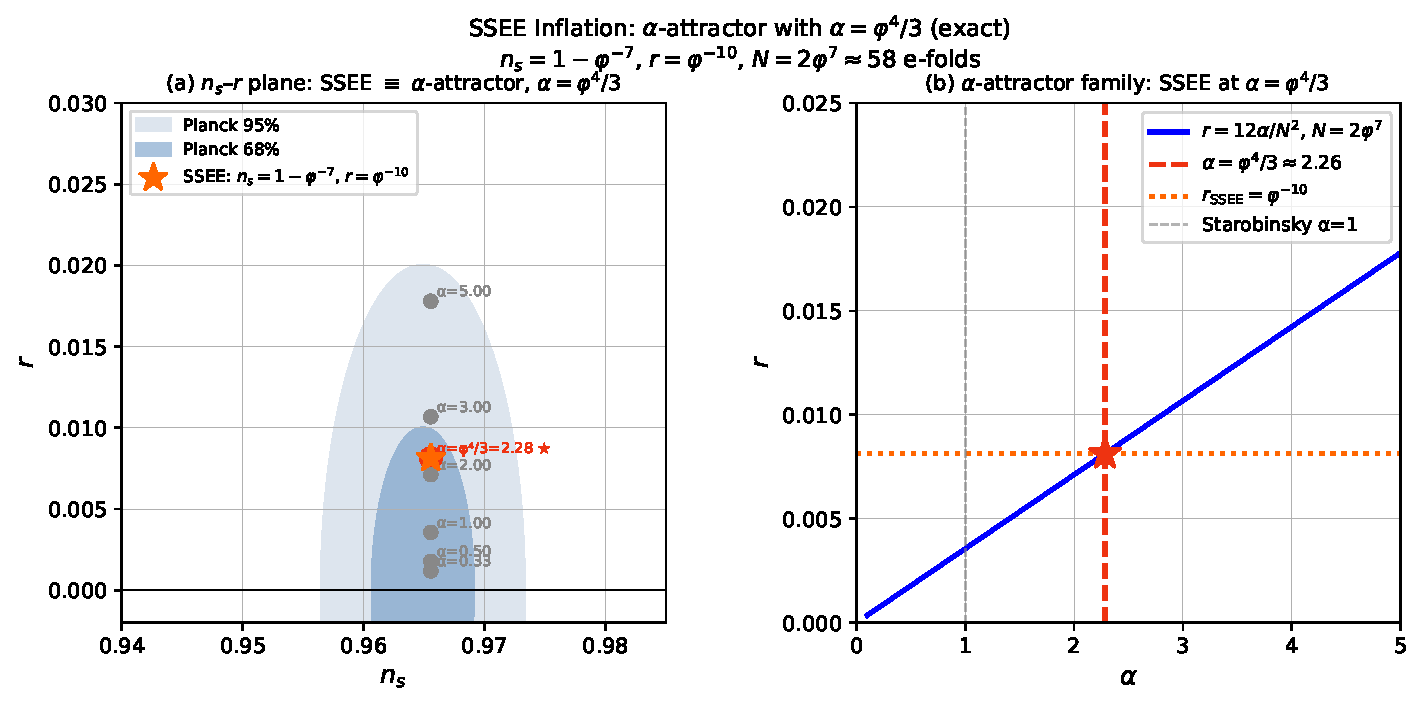
\includegraphics[width=0.85\textwidth]{../results/figures/fig_inflation_connection.pdf}
\caption{Analytical validation of the primordial tensor-to-scalar ratio $r$ against Planck constraints.}
\end{figure}

\begin{figure}[htbp]
\centering
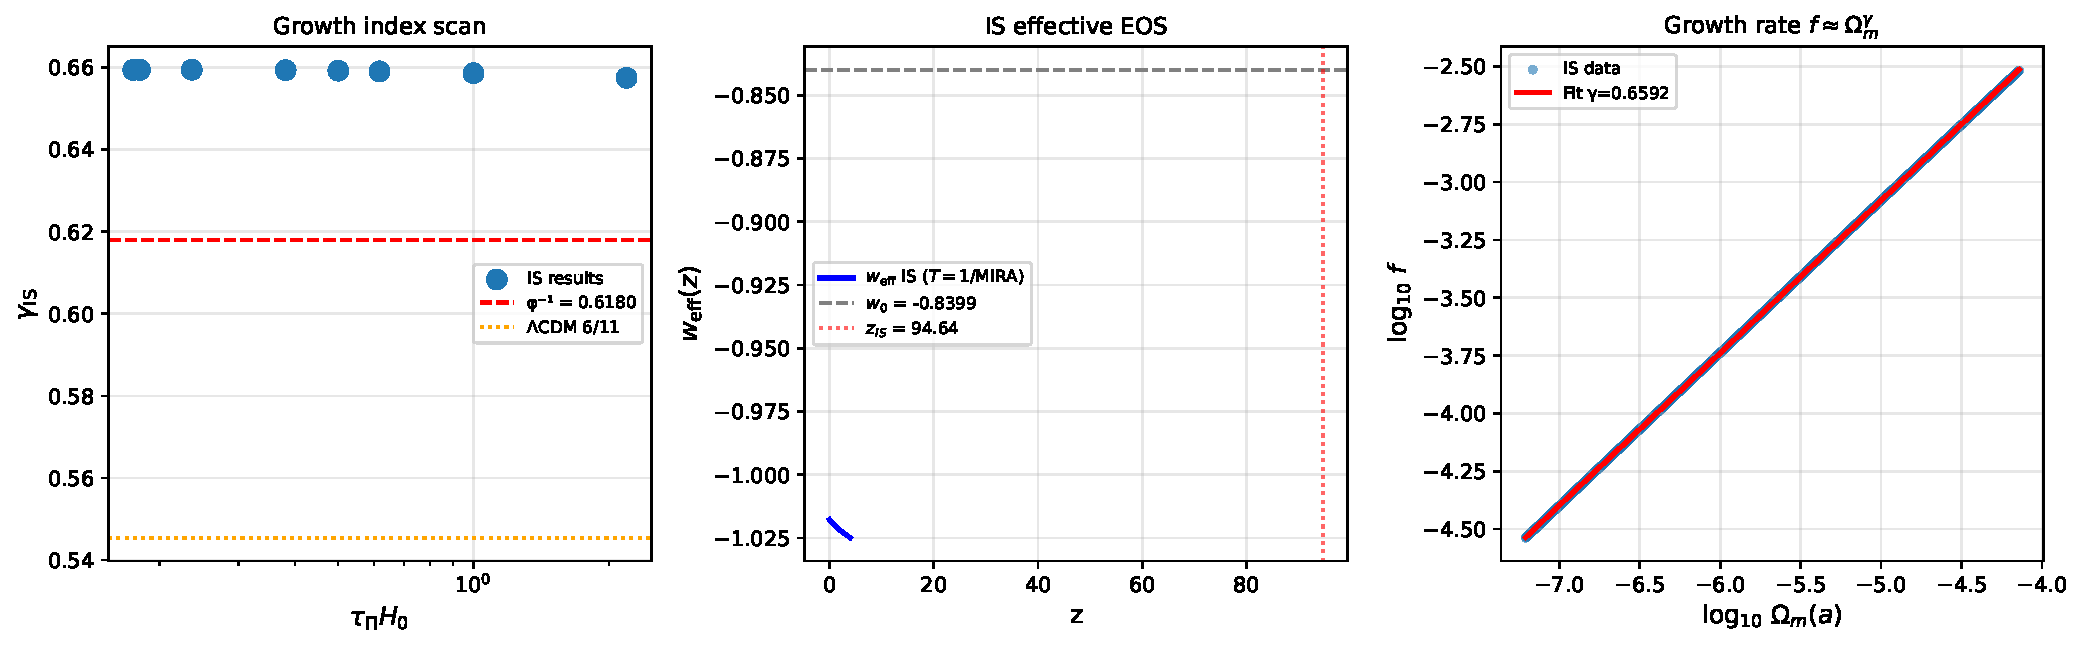
\includegraphics[width=0.85\textwidth]{../results/figures/fig_is_growth.pdf}
\caption{Israel-Stewart causal thermodynamics: prediction of the dynamical growth index and effective equation of state.}
\end{figure}

\begin{figure}[htbp]
\centering
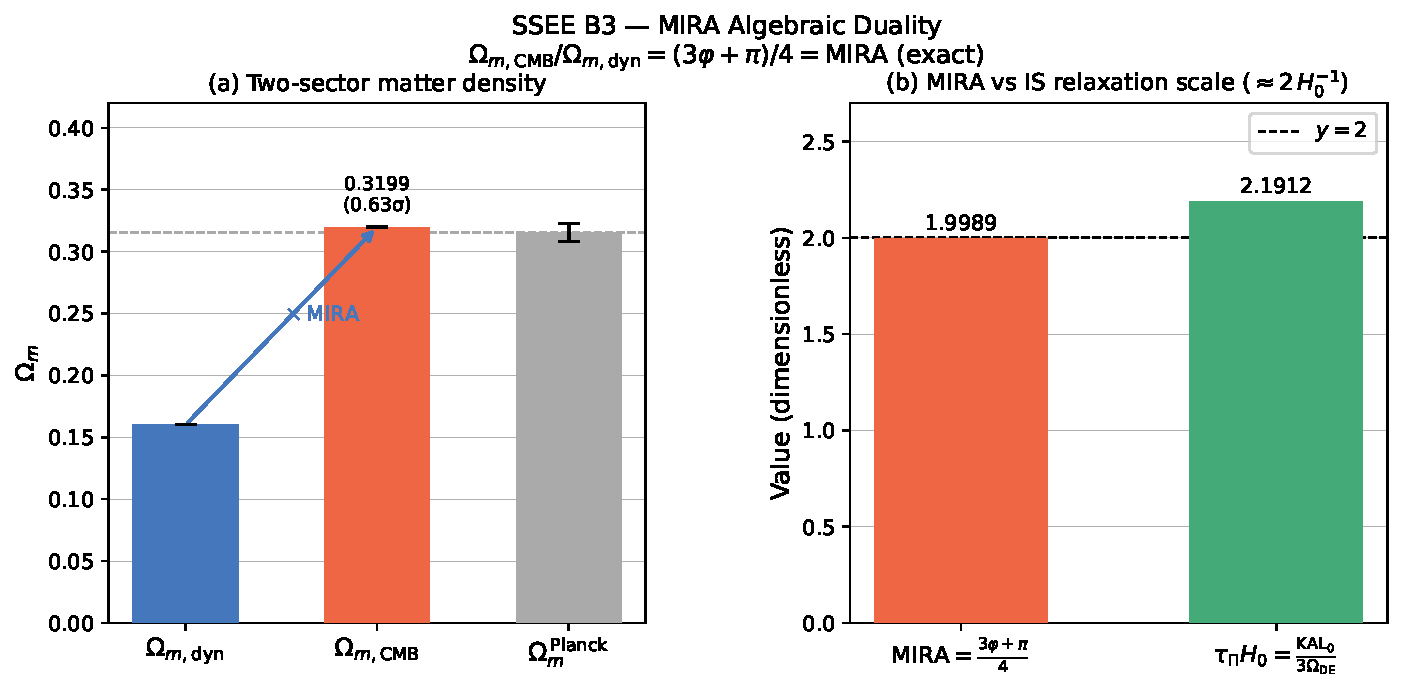
\includegraphics[width=0.85\textwidth]{../results/figures/fig_b3_mira.pdf}
\caption{MIRA geometry constraint: representation of the observational horizon scaling.}
\end{figure}

\bibliographystyle{plainnat}
\bibliography{SSEE_Paper4}

\end{document}
